
%\begin{frame}{\Titulo \footnotemark (1)}
\begin{frame}{\citetitle{MarcoNuno_CongArbEsp_2020_09_01} \footnotemark (1)}
\begin{block}{Problem description} 
\begin{itemize}
\item In Mexico, nearly 145 thousand vehicles were theft in 2020. 
\note[item]{\scriptsize These numbers include theft of an unattended vehicle without a key, the unauthorized use of a car, the removal of an unattended vehicle with the keys visible, taking a vehicle by force, or threat of force, against its owner or operator. }
\item Car thefts were consistently increasing between the period of 2015 and 2018.
 
\item The security systems in older vehicles may not be up to the same standard as newer vehicles.
\note[item]{\scriptsize We designed the proposed system for older vehicles that do not have a last-generation system, since older vehicles are straightforward to theft.} 
\item One anti-theft alternative system is a GPS tracker. 
\note[item]{\scriptsize A GPS tracking device is a portable unit that allows users to monitor and track its location.}
\begin{itemize}
\item Advantages:  Widely available. 
\item Disadvantage: Only track vehicle in real-time, but without knowing driver's identity.  
\end{itemize}
\item We propose a smartphone-based face-detection anti-theft system. 
\note[item]{\scriptsize The system used several sensors (including a smartphone's camera) to detect a theft attempt in real-time. }
\end{itemize}
\end{block} 
\footnotetext[1]{\fullcite{MarcoNuno_CongArbEsp_2020_09_01}}
\setcounter{footnote}{0}
\end{frame}




\begin{frame}{\citetitle{MarcoNuno_CongArbEsp_2020_09_01} (2)}

\begin{block}{Proposed system} 

\begin{columns}
\begin{column}{0.5\textwidth}

A security system mounted on a smartphone that continously:
	\begin{itemize}
\item Monitors passengers identity using front or rear camera of the smartphone.
\note[item]{\scriptsize The smartphone has an application that continuously detects faces, extracts features, and compares the detected faces with faces of registered passengers. }
\item Monitors the real-time vehicle's GPS localization.
\note[item]{\scriptsize This function mimics the commercial GPS trackers.}

\item Monitors the vehicle's movement using the accelerometers.
\note[item]{\scriptsize This sensor detects the car hit or when the stealing of car parts is in the process when the vehicle is parked. }

\item Informs problems to the system administrator using its own data connectivity.

\note[item]{\scriptsize The smartphone has have a separate battery that guarantees the system's functioning even when the car's main battery was disconnected. }

	\end{itemize}
\end{column}	
\begin{column}{0.5\textwidth}
	\begin{center}
     %%%%% this is a minipage, so \textwidth is already adjusted to the size of the column
     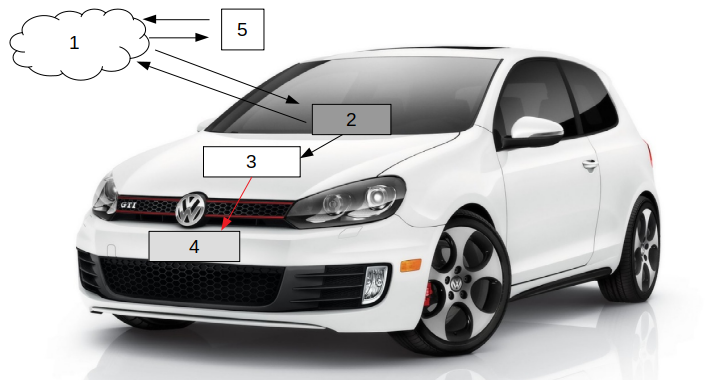
\includegraphics[width=0.99\textwidth]{Figs/ConductorAutorizado2}
     \end{center}
\end{column}		
\end{columns}	
\end{block} 
\end{frame}


\begin{frame}{\citetitle{MarcoNuno_CongArbEsp_2020_09_01} (3)}

\begin{block}{Results}
\begin{columns}
\begin{column}{0.5\textwidth}
\note[item]{\scriptsize The proposed application includes a remote mode, where the system administrator can exchange one of the two modes of operation remotlely.}
Operation modes:
	\begin{enumerate}
\item Enrollment: Faces of passenger in the car are stored and used to build a model of authorized users.
\note[item]{\scriptsize The model build is done on the device's, but the system administrator is informed of the details of this step. - He must know the number of used involved in the enrroloment. }
\item Test: Faces of passengers are analyzed and any unauthorized passenger is detected.
\note[item]{\scriptsize The system administrators takes confirms that the detected faces does not correspond to autorized passenger, and takes the decision of the action to be carried out.  }

	\end{enumerate}
Limitations:
	\begin{itemize}
\item Only passengers in the front seats and the passenger in the center of the back seat can be detected. 
\note[item]{\scriptsize One solution is to use an additional camera or to change the smarphone location.}
\item Daylight illumination.
\note[item]{\scriptsize The solution is to replace the device's camera with an IR camera. }
\item Device hiding is in an early phase.
%\note[item]{\scriptsize The smartphone is difficult to hide. }

	\end{itemize}

\end{column}
\begin{column}{0.5\textwidth}
\begin{center}
     %%%%% this is a minipage, so \textwidth is already adjusted to the size of the column
     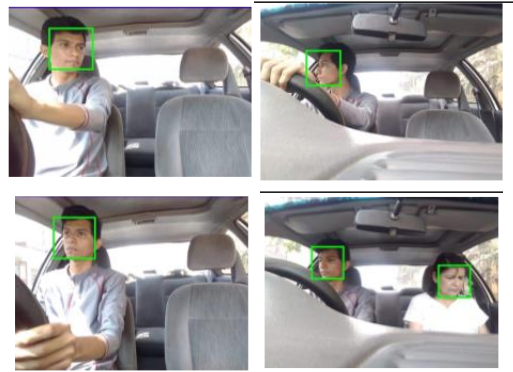
\includegraphics[width=0.99\textwidth]{Figs/ConductorAutorizado1}
     \end{center}
\end{column}

\end{columns}
\end{block} 
\end{frame}

